
\documentclass{article}

\usepackage{graphicx}

\newcommand{\di}{{d}}
\newcommand{\nexp}{{n}}
\newcommand{\nf}{{p}}
\newcommand{\vcd}{{\textbf{D}}}

\usepackage{nccmath}
\usepackage{mathtools}
\usepackage{graphicx,caption}
\usepackage{enumitem}
\usepackage{epstopdf,subcaption}
\usepackage{psfrag}
\usepackage{amsmath,amssymb,epsf}
\usepackage{verbatim}
\usepackage{url}
\usepackage[hang,flushmargin]{footmisc} 
\usepackage{hyperref}
\DeclareMathOperator*{\argmax}{arg\,max}
\DeclareMathOperator*{\argmin}{arg\,min}
\newcommand{\hurl}[1]{\href{#1}{#1}}
\renewcommand{\url}{\nolinkurl}
\AtBeginDocument{
	\label{CorrectFirstPageLabel}
	\def\fpage{\pageref{CorrectFirstPageLabel}}
}
\usepackage{color}
\usepackage{bbm}
\usepackage{listings}
\usepackage{setspace}
\usepackage{float}
\usepackage{natbib}
\definecolor{Code}{rgb}{0,0,0}
\definecolor{Decorators}{rgb}{0.5,0.5,0.5}
\definecolor{Numbers}{rgb}{0.5,0,0}
\definecolor{MatchingBrackets}{rgb}{0.25,0.5,0.5}
\definecolor{Keywords}{rgb}{0,0,1}
\definecolor{self}{rgb}{0,0,0}
\definecolor{Strings}{rgb}{0,0.63,0}
\definecolor{Comments}{rgb}{0,0.63,1}
\definecolor{Backquotes}{rgb}{0,0,0}
\definecolor{Classname}{rgb}{0,0,0}
\definecolor{FunctionName}{rgb}{0,0,0}
\definecolor{Operators}{rgb}{0,0,0}
\definecolor{Background}{rgb}{0.98,0.98,0.98}
\lstdefinelanguage{Python}{
numbers=left,
numberstyle=\footnotesize,
numbersep=1em,
xleftmargin=1em,
framextopmargin=2em,
framexbottommargin=2em,
showspaces=false,
showtabs=false,
showstringspaces=false,
frame=l,
tabsize=4,
% Basic
basicstyle=\ttfamily\footnotesize\setstretch{1},
backgroundcolor=\color{Background},
% Comments
commentstyle=\color{Comments}\slshape,
% Strings
stringstyle=\color{Strings},
morecomment=[s][\color{Strings}]{"""}{"""},
morecomment=[s][\color{Strings}]{'''}{'''},
% keywords
morekeywords={import,from,class,def,for,while,if,is,in,elif,else,not,and,or
,print,break,continue,return,True,False,None,access,as,,del,except,exec
,finally,global,import,lambda,pass,print,raise,try,assert},
keywordstyle={\color{Keywords}\bfseries},
% additional keywords
morekeywords={[2]@invariant},
keywordstyle={[2]\color{Decorators}\slshape},
emph={self},
emphstyle={\color{self}\slshape},
%
}


\pagestyle{empty} \addtolength{\textwidth}{1.0in}
\addtolength{\textheight}{0.5in}
\addtolength{\oddsidemargin}{-0.5in}
\addtolength{\evensidemargin}{-0.5in}
\newcommand{\ruleskip}{\bigskip\hrule\bigskip}
\newcommand{\nodify}[1]{{\sc #1}}
\newcommand{\points}[1]{{\textbf{[#1 points]}}}
\newcommand{\subquestionpoints}[1]{{[#1 points]}}
\newenvironment{answer}{{\bf Answer:} \sf \begingroup\color{red}}{\endgroup}%

\newcommand{\bitem}{\begin{list}{$\bullet$}%
{\setlength{\itemsep}{0pt}\setlength{\topsep}{0pt}%
\setlength{\rightmargin}{0pt}}}
\newcommand{\eitem}{\end{list}}

\setlength{\parindent}{0pt} \setlength{\parskip}{0.5ex}
\setlength{\unitlength}{1cm}

\renewcommand{\Re}{{\mathbb R}}
\newcommand{\R}{\mathbb{R}}
\newcommand{\what}[1]{\widehat{#1}}

\renewcommand{\comment}[1]{}
\newcommand{\mc}[1]{\mathcal{#1}}
\newcommand{\half}{\frac{1}{2}}

\def\KL{D_{KL}}
\def\xsi{x^{(i)}}
\def\ysi{y^{(i)}}
\def\zsi{z^{(i)}}
\def\E{\mathbb{E}}
\def\calN{\mathcal{N}}
\def\calD{\mathcal{D}}

\newcommand{\diag}{\mathop{\rm diag}}

\usepackage{tikz}
\usepackage{bbding}
\usepackage{pifont}
\usepackage{wasysym}
\usepackage{amssymb,amsthm}
\usepackage{booktabs}
\usepackage{verbatim}


\newtheorem{lemma}{Lemma}
\usepackage[utf8]{inputenc}
% \usepackage{indentfirst}
\usepackage{hyperref}
\usepackage{cite}
\usepackage[a4paper, total={6in, 10in}]{geometry}


\title{% 
    CS 229 Project Milestone \\
    Project Category: Physical Sciences \\
    Modelling State-of-Health for a Li-ion Battery}
\author{Karthik Nataraj (kartnat), Hampus Carlens (hcarlens) and Julian Cooper (jelc)}
\date{\today}

\begin{document}

\maketitle


Format\\
Your milestone should be at most 3 pages, excluding references. Similar to the proposal, it should include
- Motivation: What problem are you tackling, and what's the setting you're considering?
Method: What machine learning techniques have you tried and why?\\

- Preliminary experiments: Describe the experiments that you've run, the outcomes, and any error analysis that you've done. You sould have tried at least one baseline.\\

- Next steps: Given your preliminary results, what are the next steps that you're considering?


\section{Motivation}
Lithium ion batteries are of great and increasing importance in today's society due to their high energy density. We are very dependent on their performance. Li-on batteries' performance capability can be characterized by their so called state of health (SOH). SOH is a measure of usable capacity over rated capacity. Accurately predicting how many cycles (i.e charge - discharge) a battery can perform, at any given time, before reaching it’s end of useful life is difficult, however important for reliability etc. 

The predicting is hard in part due to poor understanding of how the measurable parameters (voltage, current etc) effect the SOH. Today three main methods; electrochemical models, equivalent circuit models and data-driven models, are used.

We aim to use a data-driven model to predict remaining useful life (RUL) and future SOH degradation. This method requires little knowledge about the underlying factors. There have been previous studies successfully achieving data driven SOH prediction with high accuracy. For example some recognized studies are \cite{severson2019data}, \cite{roman2021machine} and \cite{energiesMdpi}. These articles show predictions of SOH and RUL with over 90\% accuracy. The highest accuracies are obtained using deep neural networks such as in \cite{roman2021machine} and \cite{energiesMdpi}. There, accuracies $>97\%$ have been reported. However, the authors of \cite{energiesMdpi} and \cite{DariusOld} point toward the importance of future work in trying to scale the models, to make them suitable for front-end embedded systems. In \cite{severson2019data} they attempt to not use deep learning and use a linear model instead. They achieved a significantly lower accuracy and resolution of the predictions, mainly being able to predict RUL using a lot of cycles. We specifically aim to query the interactions learned by the neural network model (SHAP, LIME, etc.) to infer complex features we might use to build a simpler, explainable white-box model with reasonable accuracy. The model should be able to predict SOH using fewer cycles than \cite{severson2019data} and with higher accuracy.


\section{Method}
We can classify our approaches into two categories, black-box and white-box methods: WORK IN PROGRESS ...

\subsection{Black-box model}
These include sequential deep learning techniques such as RNN's and LSTM networks, which we can use to predict the decay curves of capacity versus cycle number based on a feature set including various voltage, current, and temperature information. 

\subsection{White-box model}
Various autoregressive models, feature engineering based on assessment of black box model with target being the SoH or “capacity” (number of hours for which a battery can provide a current equal to the discharge rate at battery’s rated voltage).

Since we ultimately want to use early cycle information to predict the exact decay curve, it might be the case that the sequential neural networks will not have enough information--in this case we may revert to regular dense, fully connected layers, which have the added benefit of easily incorporating other features.  
%In the Nature paper mentioned in the data source below, the only method used was a regularized linear model.  Models using information from previous cycles to predict the SoH at the current cycle were ignored due to poor correlations between SoH at early cycles and% 


\section{Data exploration}
The \href{https://data.matr.io/1/projects/5c48dd2bc625d700019f3204}{dataset} we have selected contains approximately 96,700 cycles (approx. 780 cycles per battery for 124 batteries). For each cycle we capture voltage, current applied and temperature sampled at 2.5 second intervals. This is largest publicly available for nominally identical commercial lithium-ion batteries cycled under controlled conditions, and is the same source used by two recent papers that motivated our project: “Machine learning pipeline for battery state-of-health estimation” (Nature, 2021)\cite{roman2021machine} and "Data-driven prediction of battery cycle life before capacity degradation" (Nature, 2019)\cite{severson2019data}.

\begin{itemize}
    \item \textbf{Discharge capacity vs cycle number}. Our goal is to predict the discharge curves below given information from the first 50-100 cycles. A few things to note. First, the batteries in our population are either rated at 1.1 Ah or 1.05 Ah nominal capacity. By nominal here we mean manufacturer rated initial capacity. Second, in practice, our initial discharge capacity rarely perfectly matches the nominal capacity rating and so instead of two discrete starting points at 1.1 and 1.05, our starting points range continuously in that range. Third, our data is meant to reflect cycling each battery from its initial capacity to 80\% of its nominal. This explains the two distinct end points we observe in the right hand chart at 0.88 Ah and 0.84 Ah, the 80\% thresholds of 1.1 Ah and 1.05 Ah nominal capacities respectively. Last, in plotting these curves we identified some obvious outliers. Batteries in the left hand plot with capacities either above 1.2 or below 0.8 are erroneous measurements that we remove from the data before training.  

        \begin{figure}[H]
            \centering
            \begin{subfigure}[b]{0.49\linewidth}
                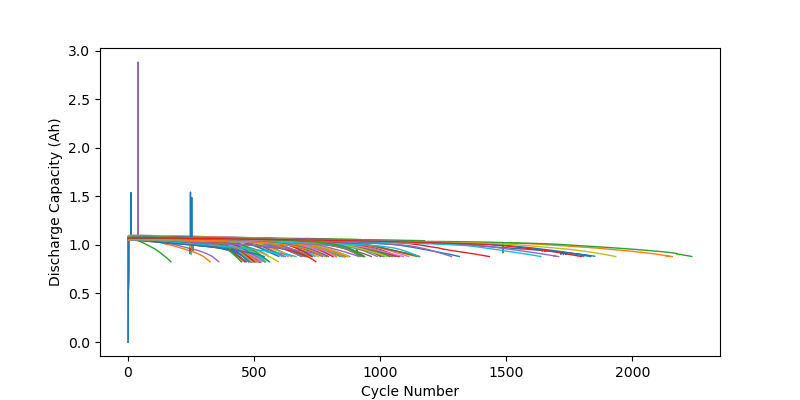
\includegraphics[width=\linewidth]{figs/discharge_capacity_by_cycle.png}
                \caption{Complete dataset}
            \end{subfigure}
            \begin{subfigure}[b]{0.49\linewidth}
                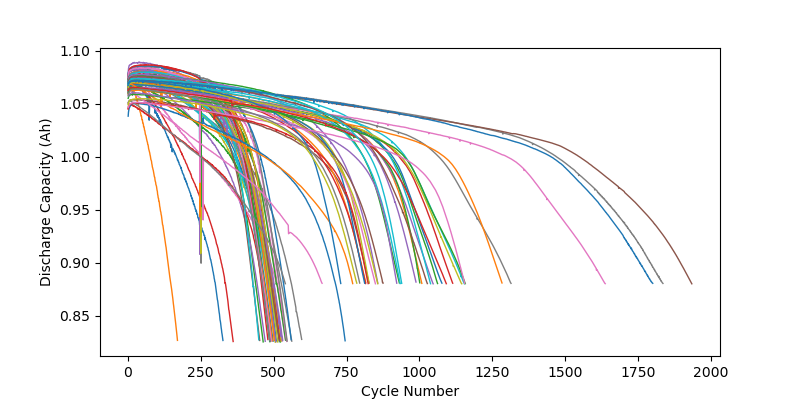
\includegraphics[width=\linewidth]{figs/discharge_capacity_by_cycle_remove_outliers.png}
                \caption{Outliers removed}
            \end{subfigure}
            \caption{Discharge capacity by cycle number for 124 batteries}
            \label{fig:3a}
        \end{figure}

    \item \textbf{Distribution of our target variable}. Cycle life is the number of cycle it takes for a given battery to reach 80\% of its nominal capacity. This is our target variable. When plotting the complete dataset we identified a skewed normal distribution. Ideally we want to roughly maintain this distribution for our validation and test data. To achieve this we re-used logic from "Data-driven prediction of battery cycle life before capacity degradation" (Nature, 2019)\cite{severson2019data} to split our train, validation and test data.

        \begin{figure}[H]
            \centering
            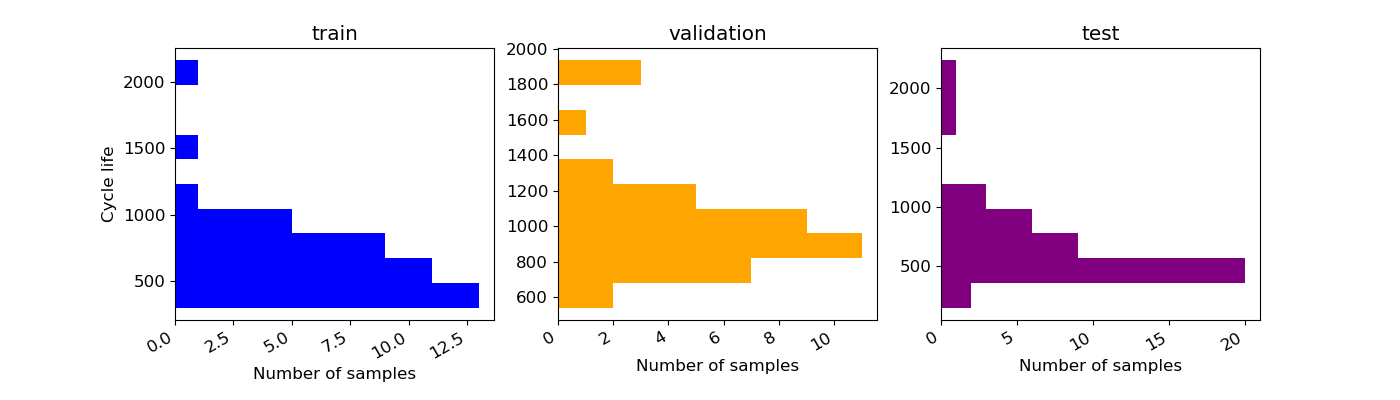
\includegraphics[scale=0.5] {figs/histogram_cycle_life_traintest.png}
            \caption{Distribution of target for train, validation and test data}
            \label{fig:1b}
        \end{figure}

    \item \textbf{Applied current and charge cycle}. The charts below illustrate current and positive / negative charge for all cycles of an example battery data point (ref: c1b0). We can immediately confirm that the vast majority of cycles follow similar charge profiles. In particular, applying positive current (charging) for first 500-700 time steps, then switching to an applied negative current (discharging) until depleted at the end of the cycle. The positive (Qc) and negative (Qd) charge plots also show this transition, with Qc increasing up until the changeover to negative applied current, and Qd increasing only after the changeover.

            \begin{figure}[H]
            \centering
            \begin{subfigure}[b]{0.32\linewidth}
                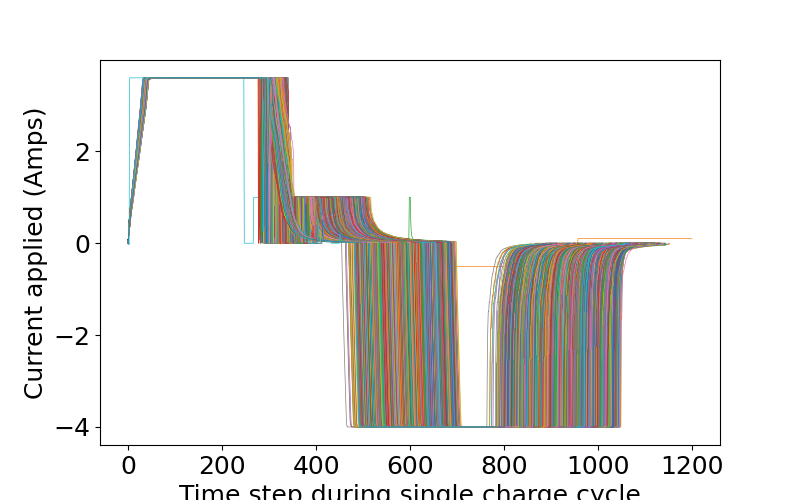
\includegraphics[width=\linewidth]{figs/b1c0_iapp_intracycle.png}
                \caption{Applied current}
            \end{subfigure}
            \begin{subfigure}[b]{0.32\linewidth}
                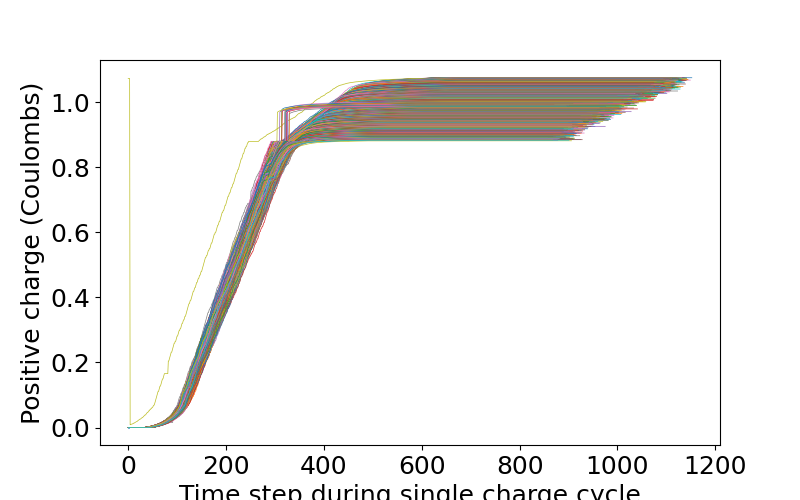
\includegraphics[width=\linewidth]{figs/b1c0_qc_intracycle.png}
                \caption{Positive charge (Qc)}
            \end{subfigure}
            \begin{subfigure}[b]{0.32\linewidth}
                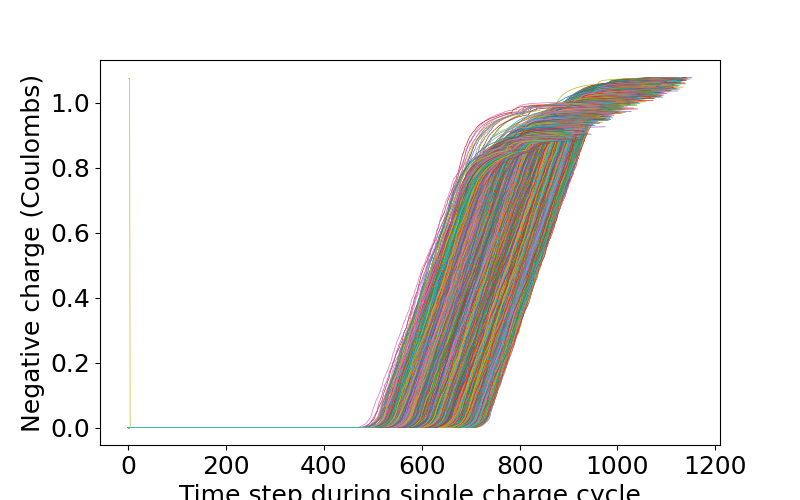
\includegraphics[width=\linewidth]{figs/b1c0_qd_intracycle.png}
                \caption{Negative charge (Qd)}
            \end{subfigure}
            \caption{Charge and discharge cycles for an example battery (ref: b1c0)}
            \label{fig:1c}
        \end{figure}

    We also investigated how voltage and temperature vary over the cycles of the same example battery. It is interesting to note that while temperature has a roughly gaussian distribution throughout any given cycle, the voltage measure has almost no variance during charge but significant variance across cycles during discharge. 
    
        \begin{figure}[H]
            \centering
            \begin{subfigure}[b]{0.49\linewidth}
                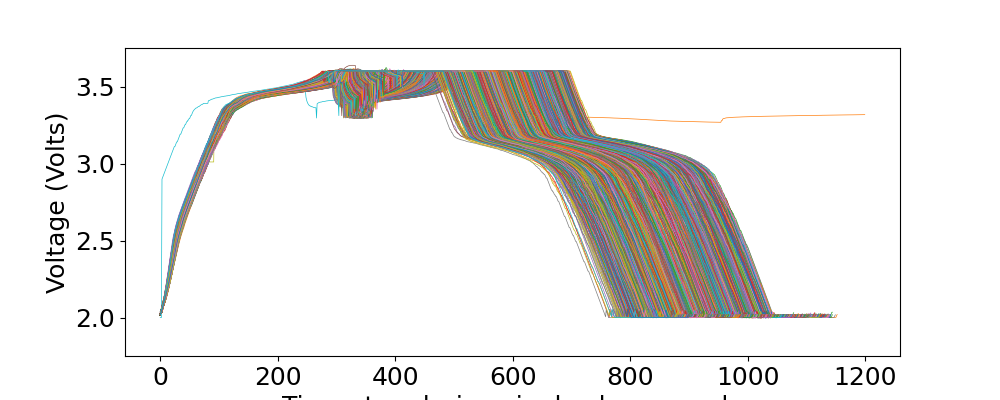
\includegraphics[width=\linewidth]{figs/b1c0_voltage_intracycle.png}
                \caption{Voltage (volts)}
            \end{subfigure}
            \begin{subfigure}[b]{0.49\linewidth}
                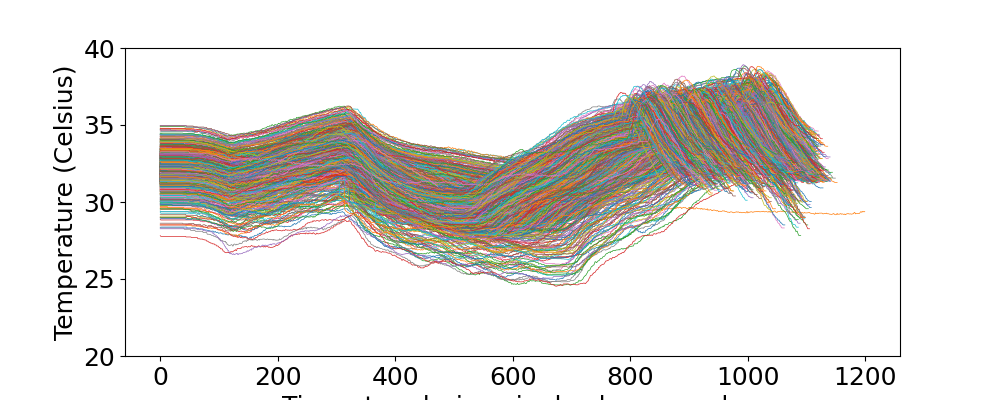
\includegraphics[width=\linewidth]{figs/b1c0_temp_intracycle.png}
                \caption{Temperature (degrees celsius)}
            \end{subfigure}
            \caption{Voltage and temperature over cycles for an example batter (ref: b1c0)}
            \label{fig:1d}
        \end{figure}
        
    \item \textbf{Correlation with cycles @ 5\% fade}. Finally, we wanted to directly plot some measure of capacity fade (in this case number of cycles to reach 5\% decrease from nominal) during the initial cycles against cycle life to see if we can recover the correlated behaviour we expect between early trajectory and end point of the discharge capacity curve. Encouragingly, we see the two are highly correlated, achieving a pearson correlation coefficient of approximately 0.94.

        \begin{figure}[H]
            \centering
            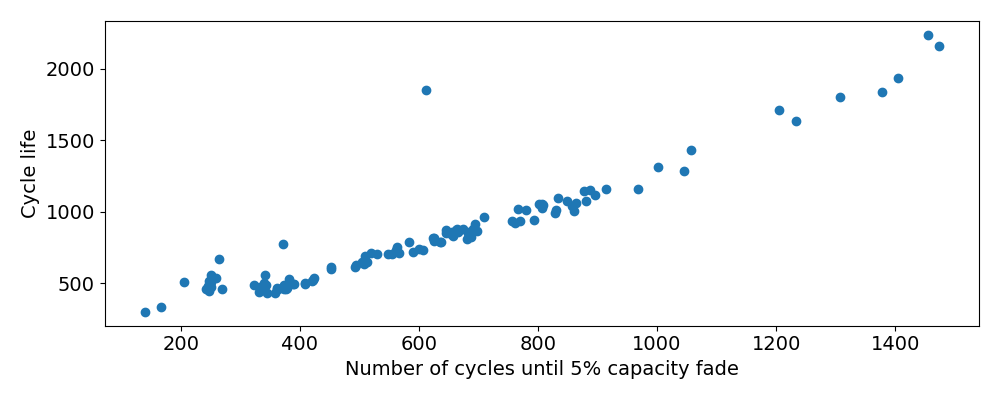
\includegraphics[scale=0.7] {figs/correlation_cycle_life_vs_5pct_fade.png}
            \caption{Scatter plot demonstrating correlation between cycle life and 5\% capacity fade}
            \label{fig:1e}
        \end{figure}

\end{itemize}


\section{Experiments}
\subsection{Model fit evaluation}

Our plan is to use ~70\% of the data for training, leaving ~15\% for cross-validation and ~15\% for out-of-sample validation. For out-of-sample validation we will initialize with the first 10 cycles, and then ask the model to predict State-of-Health (SOH) for the next 90 cycles (or until we hit end-of-life threshold).

To evaluate out-of-sample performance, we will compute two error metrics:
\begin{enumerate}
    \item \textbf{State-of-Health (SOH)}: Compute Mean Squared Error for predicted SOH values, one value per cycle for each battery used for validation. 
    \item \textbf{Remaining-Useful-Life (RUL)}: Compute Mean Squared Error for predicted RUL values, one value per battery used for validation.
\end{enumerate}

While these error metrics are related (RUL = first cycle for which SOH dips below end-of-life threshold), they do measure different things. For example, we might correctly predict the number of cycles before end-of-life (let's say 100), but guess that the path is linear instead of parabolic or logistic. This might mean that at 50 cycles our prediction of available capacity (SOH) is much worse than the true value despite good RUL accuracy. 

\subsection{Prediction and inference}

Our goal is to build two models: one for prediction and the other for inference:
\begin{enumerate}
    \item \textbf{Prediction}: Black-box model (e.g., LSTM Neural Network) that is intended to be a useful tool for battery manufacturers to test (predict RUL and SOH profile given 10 cycles) their batteries meet desired capacity specifications before leaving the factory. 
    \item \textbf{Inference}: By querying the results of our black box model (e.g., partial dependence plots) we hope to learn the marginal effects of our feature variables. Given this and our understanding of the battery physics, we would like to construct a alternative white box model (e.g., Auto-regression) from which we can perform inference
\end{enumerate}

Given what we learn from our initial black box model, we hope to develop a white box model which comparable performance metrics. Such a model is often more desirable for engineering applications since its relationships and behavior are transparent and simple to sense check against known physics.


% \section{Appendix}
% \subsection{Supplementary data exploration}
% WORK IN PROGRESS ...

\bibliographystyle{IEEEtran}

\bibliography{citation}

\end{document}
